\documentclass[11pt,a4paper]{article}

\usepackage[margin=1in]{geometry}
\usepackage{booktabs}
\usepackage{graphicx}
\usepackage{hyperref}
\usepackage{xcolor}
\usepackage{listings}
\usepackage{amsmath}
\usepackage{tikz}
\usetikzlibrary{arrows.meta, positioning, shapes.geometric, fit}

\definecolor{codebg}{RGB}{245,245,245}
\lstset{
  basicstyle=\ttfamily\small,
  backgroundcolor=\color{codebg},
  breaklines=true,
  frame=single,
  framesep=4pt,
  columns=fullflexible
}

\title{4-Bit GPTQ Quantization Pipeline for OpenVLA:\\File Reference and Architecture}
\author{VLA Memory Bench}
\date{\today}

\begin{document}
\maketitle

\begin{abstract}
This document describes the file structure and data flow of the 4-bit GPTQ quantization pipeline used to evaluate OpenVLA models on the LIBERO robot manipulation benchmark. It covers quantization, inference, evaluation, and analysis stages.
\end{abstract}

\tableofcontents
\newpage

%% ====================================================================
\section{Overview}

The pipeline takes four OpenVLA models finetuned on LIBERO suites, quantizes their LLM backbone from fp16 to 4-bit GPTQ, evaluates them in closed-loop robot control, and analyzes the resulting trajectories. The key insight is that \textbf{only the LLM backbone} (Llama-2-7B, $\sim$7B parameters) is quantized; the vision encoder (DinoSigLIP) and projector remain in fp16 because they are small and sensitive to quantization.

Model size drops from $\sim$14\,GB (fp16) to $\sim$4\,GB (4-bit GPTQ) per checkpoint.

%% ====================================================================
\section{File Reference}

\subsection{Quantization}

\begin{table}[h]
\centering
\begin{tabular}{@{}p{5.5cm}p{9cm}@{}}
\toprule
\textbf{File} & \textbf{Purpose} \\
\midrule
\texttt{quantize\_checkpoints.py} & Master quantization script. Downloads fp16 OpenVLA checkpoints from HuggingFace, extracts the LLM backbone, runs GPTQ quantization with 128 calibration samples, and saves the result. Vision encoder weights are saved separately in fp16. \\
\bottomrule
\end{tabular}
\caption{Quantization stage (single file).}
\end{table}

\paragraph{Key functions in \texttt{quantize\_checkpoints.py}:}
\begin{description}
  \item[\texttt{register\_openvla()}] Registers custom OpenVLA model classes with HuggingFace's \texttt{AutoModel} so the checkpoint can be loaded.
  \item[\texttt{create\_calibration\_data()}] Generates 128 LIBERO-style text prompts (e.g., \textit{``In: What action should the robot take to pick up the black bowl...? Out:''}) used by GPTQ to calibrate weight quantization.
  \item[\texttt{quantize\_model()}] End-to-end pipeline: load model $\rightarrow$ extract LLM $\rightarrow$ save vision weights $\rightarrow$ run GPTQ $\rightarrow$ save metadata.
\end{description}

\subsection{Quantized Checkpoint Structure}

Each quantized checkpoint lives under \texttt{checkpoints/} and contains:

\begin{table}[h]
\centering
\begin{tabular}{@{}p{6.5cm}p{8cm}@{}}
\toprule
\textbf{File / Directory} & \textbf{Contents} \\
\midrule
\texttt{config.json}               & Full OpenVLA model config including \texttt{norm\_stats} (per-suite action mean/std for denormalization). \\
\texttt{quantize\_config.json}     & GPTQ metadata: bits=4, group\_size=128, quantization time. \\
\texttt{non\_llm\_weights.pt}      & Vision encoder + projector weights in fp16 ($\sim$1.6\,GB). \\
\texttt{llm\_quantized/}           & Directory containing the quantized LLM. \\
\quad \texttt{gptq\_model-4bit-128g.safetensors} & Quantized Llama-2-7B weights ($\sim$3.9\,GB). \\
\quad \texttt{config.json}         & Llama-2-7B config with \texttt{quantization\_config} block. \\
\quad \texttt{quantize\_config.json} & GPTQ parameters (bits, group\_size, damp\_percent=0.1). \\
\texttt{tokenizer.json}            & Llama tokenizer. \\
\texttt{preprocessor\_config.json} & Image processor config ($224\times224$). \\
\texttt{norm\_stats.json}          & Action normalization statistics per LIBERO suite. \\
\bottomrule
\end{tabular}
\caption{Contents of each checkpoint directory, e.g.\ \texttt{checkpoints/openvla-7b-finetuned-libero-spatial-gptq-4bit/}.}
\end{table}

\subsection{Inference and Evaluation}

\begin{table}[h]
\centering
\begin{tabular}{@{}p{5cm}p{9.5cm}@{}}
\toprule
\textbf{File} & \textbf{Purpose} \\
\midrule
\texttt{libero\_runner\_gptq.py} & Single-task GPTQ evaluation. Loads the quantized checkpoint, runs closed-loop control in a LIBERO environment, and saves per-episode trajectories (actions, rewards, success, entropy, wall time) as JSON. \\
\texttt{run\_all\_gptq.py} & Multi-GPU batch orchestrator. Distributes 4 suites across GPUs using \texttt{ProcessPoolExecutor}, running all 10 tasks per suite sequentially on each GPU. Skips already-completed tasks. \\
\midrule
\texttt{libero\_runner.py} & Baseline runner: loads fp16 (bf16) OpenVLA from HuggingFace without quantization. Same evaluation protocol. \\
\texttt{libero\_runner\_quant.py} & Baseline runner: loads OpenVLA with bitsandbytes on-the-fly quantization (4-bit or 8-bit). Slower than GPTQ at inference. \\
\texttt{run\_all.py} & Batch runner for non-GPTQ baselines. \\
\bottomrule
\end{tabular}
\caption{Inference and evaluation scripts.}
\end{table}

\paragraph{Key functions in \texttt{libero\_runner\_gptq.py}:}
\begin{description}
  \item[\texttt{load\_openvla\_gptq()}] Reassembles the model: loads the processor, creates an OpenVLA shell, swaps in the GPTQ-quantized LLM via \texttt{AutoGPTQForCausalLM}, loads the fp16 vision weights, and reads \texttt{norm\_stats}.
  \item[\texttt{preprocess\_libero\_image()}] Rotates the image 180\textdegree\ (LIBERO renders upside-down), JPEG round-trips it (to match RLDS training), resizes to $224\times224$ with Lanczos, and optionally center-crops.
  \item[\texttt{get\_action()}] Formats the instruction as a prompt, calls \texttt{model.predict\_action()} with greedy decoding, and denormalizes the 7D action vector.
  \item[\texttt{run\_episode()}] Closed-loop controller: resets the env, waits 10 stabilization steps, then runs up to \texttt{max\_steps} of predict$\rightarrow$act$\rightarrow$observe.
\end{description}

\subsection{Results}

All GPTQ results are stored under \texttt{results/gptq\_4bit/}:

\begin{table}[h]
\centering
\begin{tabular}{@{}p{6cm}p{8.5cm}@{}}
\toprule
\textbf{File Pattern} & \textbf{Contents} \\
\midrule
\texttt{libero\_\{suite\}\_task\{id\}.json} & Per-task result file (40 total: 4 suites $\times$ 10 tasks). Contains episode-level data: action sequences, rewards, entropies, success flag, step count, wall time. \\
\texttt{aggregate.json} & Summary statistics: per-suite success rate, mean steps, mean wall time, and per-task breakdowns. \\
\bottomrule
\end{tabular}
\caption{Result files.}
\end{table}

\subsection{Analysis and Visualization}

\begin{table}[h]
\centering
\begin{tabular}{@{}p{4.5cm}p{10cm}@{}}
\toprule
\textbf{File} & \textbf{Purpose} \\
\midrule
\texttt{plot\_results.py} & Generates degradation curves (TSR vs.\ horizon), per-task bar charts, and action entropy traces. Outputs PNG plots. \\
\texttt{analyze\_episodes.py} & Within-episode signal analysis: computes action magnitude, action repetition, gripper oscillation, and action diversity over time. Compares success vs.\ failure episodes. \\
\texttt{classify\_failures.py} & Failure mode classifier. Categorizes failed episodes into: \textsc{Gripper Indecision} (45\%), \textsc{Grasp Lost} (31\%), \textsc{Stalled} (28\%), \textsc{Stuck Loop} (14\%), \textsc{Aimless Wandering} (12\%). Outputs JSON labels and a summary report. \\
\bottomrule
\end{tabular}
\caption{Analysis scripts.}
\end{table}

%% ====================================================================
\section{Pipeline Data Flow}

\begin{figure}[h]
\centering
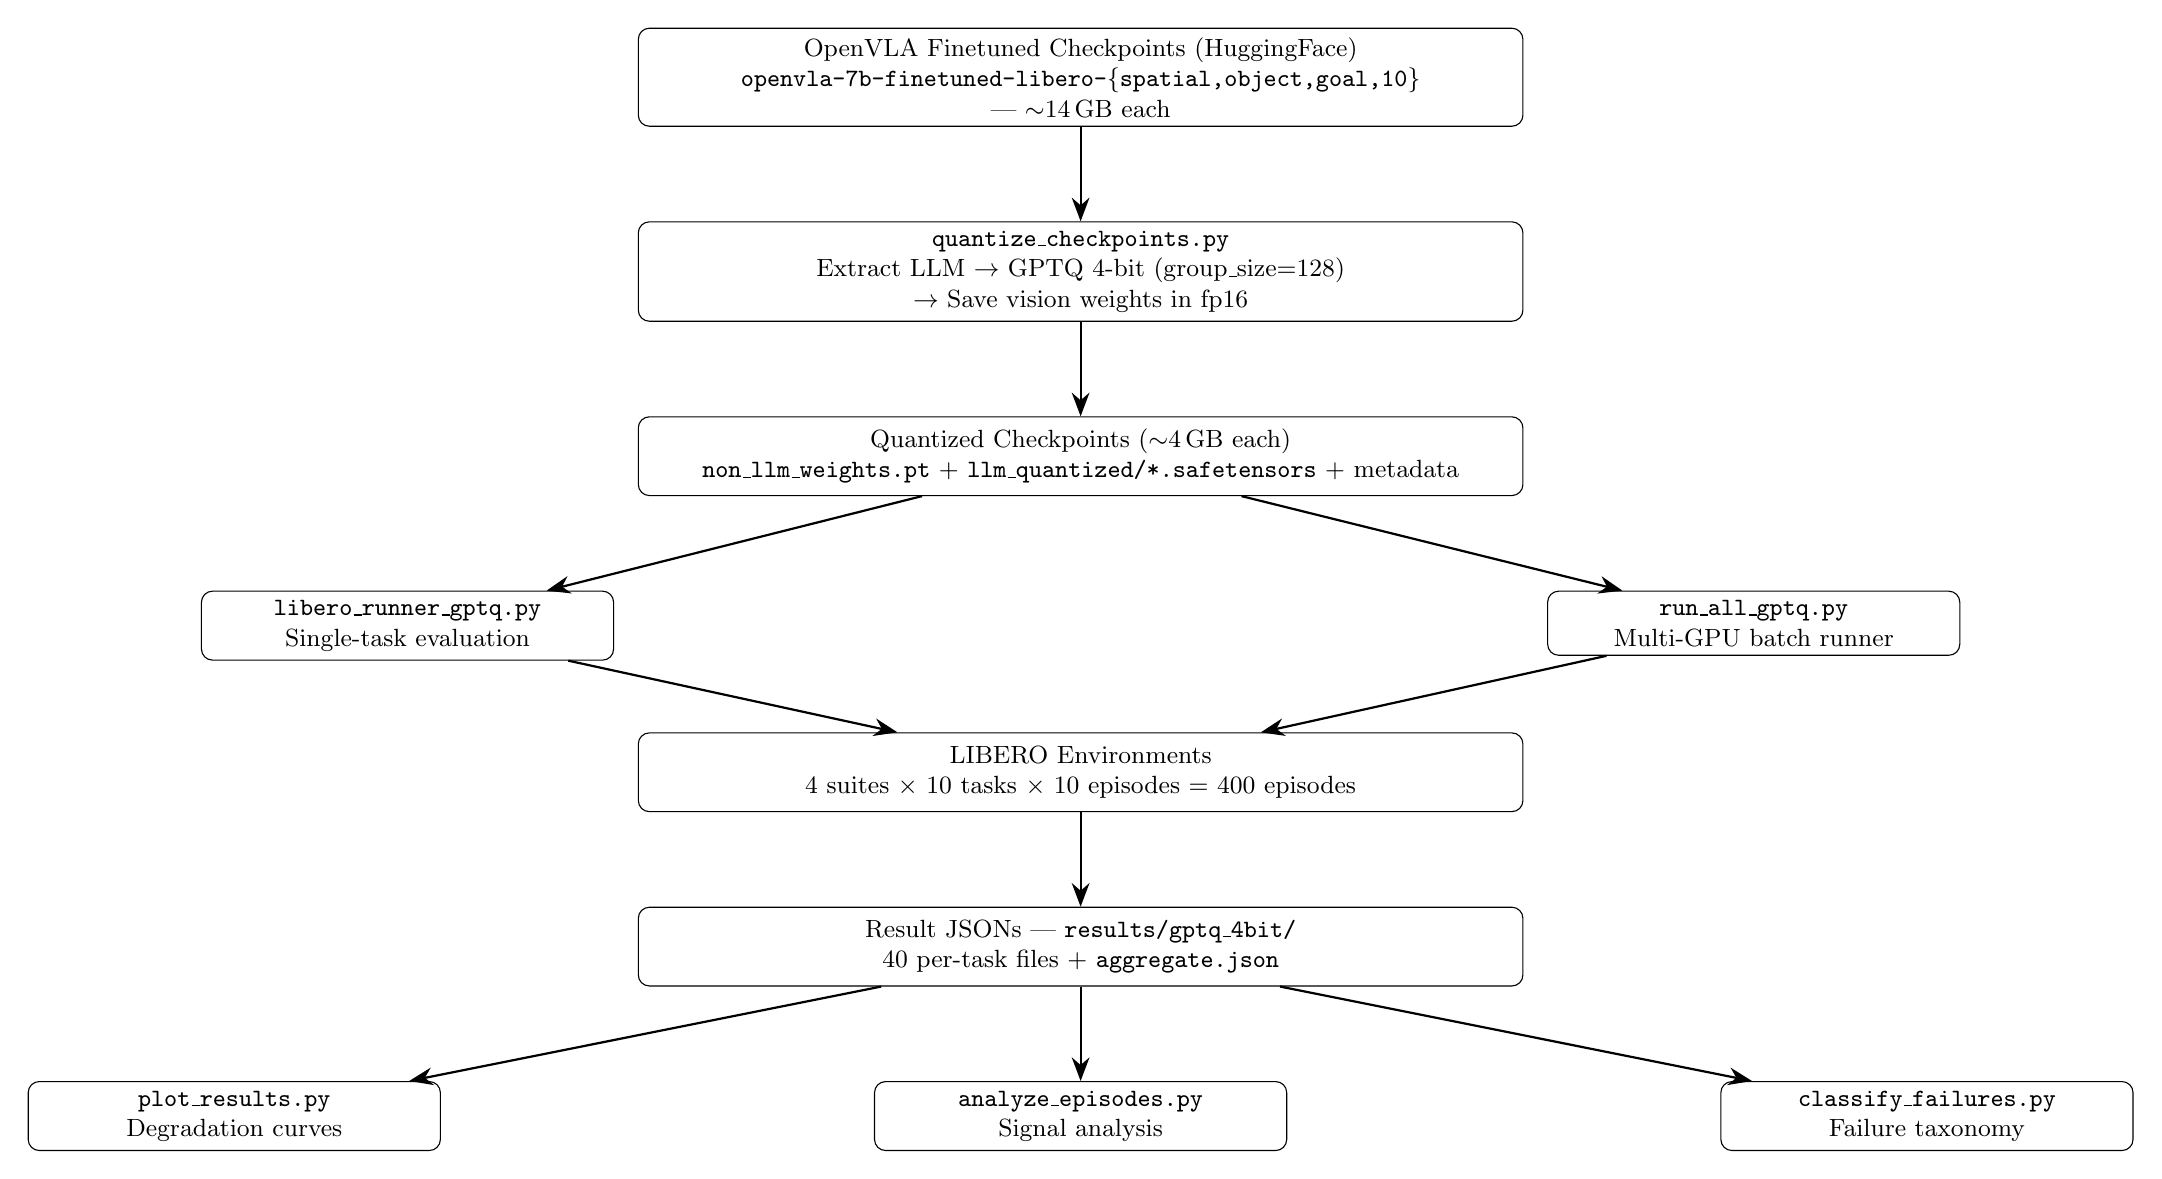
\begin{tikzpicture}[
    node distance=1.2cm and 0.5cm,
    block/.style={rectangle, draw, rounded corners, text width=11cm,
                  minimum height=1cm, align=center, font=\small},
    smallblock/.style={rectangle, draw, rounded corners, text width=5cm,
                       minimum height=0.8cm, align=center, font=\small},
    arrow/.style={-{Stealth[length=3mm]}, thick}
]
  \node[block] (hf)
    {OpenVLA Finetuned Checkpoints (HuggingFace)\\
     \texttt{openvla-7b-finetuned-libero-\{spatial,object,goal,10\}} --- $\sim$14\,GB each};

  \node[block, below=of hf] (quant)
    {\texttt{quantize\_checkpoints.py}\\
     Extract LLM $\rightarrow$ GPTQ 4-bit (group\_size=128) $\rightarrow$ Save vision weights in fp16};

  \node[block, below=of quant] (ckpt)
    {Quantized Checkpoints ($\sim$4\,GB each)\\
     \texttt{non\_llm\_weights.pt} + \texttt{llm\_quantized/*.safetensors} + metadata};

  \node[smallblock, below left=1.2cm and 0.3cm of ckpt] (single)
    {\texttt{libero\_runner\_gptq.py}\\Single-task evaluation};

  \node[smallblock, below right=1.2cm and 0.3cm of ckpt] (batch)
    {\texttt{run\_all\_gptq.py}\\Multi-GPU batch runner};

  \node[block, below=3cm of ckpt] (env)
    {LIBERO Environments\\
     4 suites $\times$ 10 tasks $\times$ 10 episodes = 400 episodes};

  \node[block, below=of env] (results)
    {Result JSONs --- \texttt{results/gptq\_4bit/}\\
     40 per-task files + \texttt{aggregate.json}};

  \node[smallblock, below left=1.2cm and 2.5cm of results] (plot)
    {\texttt{plot\_results.py}\\Degradation curves};

  \node[smallblock, below=1.2cm of results] (analyze)
    {\texttt{analyze\_episodes.py}\\Signal analysis};

  \node[smallblock, below right=1.2cm and 2.5cm of results] (classify)
    {\texttt{classify\_failures.py}\\Failure taxonomy};

  \draw[arrow] (hf) -- (quant);
  \draw[arrow] (quant) -- (ckpt);
  \draw[arrow] (ckpt) -- (single);
  \draw[arrow] (ckpt) -- (batch);
  \draw[arrow] (single) -- (env);
  \draw[arrow] (batch) -- (env);
  \draw[arrow] (env) -- (results);
  \draw[arrow] (results) -- (plot);
  \draw[arrow] (results) -- (analyze);
  \draw[arrow] (results) -- (classify);
\end{tikzpicture}
\caption{End-to-end pipeline data flow.}
\end{figure}

%% ====================================================================
\section{Quantization Parameters}

\begin{table}[h]
\centering
\begin{tabular}{@{}lll@{}}
\toprule
\textbf{Parameter} & \textbf{Value} & \textbf{Note} \\
\midrule
Method           & GPTQ           & Fast GPU inference kernels \\
Bits             & 4              & $\sim$3.5$\times$ memory reduction \\
Group size       & 128            & Block size for weight quantization \\
Damp percent     & 0.1            & Damping for Hessian inversion \\
Desc act         & False          & No per-channel activation ordering \\
Calibration samples & 128--256    & LIBERO-style text prompts \\
Vision precision & float16        & DinoSigLIP encoder kept in fp16 \\
Image size       & $224\times224$ & Input to vision encoder \\
\bottomrule
\end{tabular}
\caption{GPTQ quantization hyperparameters.}
\end{table}

%% ====================================================================
\section{Evaluation Results Summary}

\begin{table}[h]
\centering
\begin{tabular}{@{}lccccc@{}}
\toprule
\textbf{Suite} & \textbf{Horizon} & \textbf{Tasks} & \textbf{Episodes} & \textbf{Success Rate} & \textbf{Mean Steps} \\
\midrule
\texttt{libero\_spatial} & Short (10--20)       & 10 & 100 & \textbf{83\%} & 129.3 \\
\texttt{libero\_object}  & Medium (20--50)      &  9 &  90 & 69\%          & 200.8 \\
\texttt{libero\_goal}    & Med-long (30--80)    & 10 & 100 & 75\%          & 164.7 \\
\texttt{libero\_10}      & Long (50--100+)      &  9 &  90 & 47\%          & 408.7 \\
\bottomrule
\end{tabular}
\caption{4-bit GPTQ evaluation results across LIBERO suites. Performance degrades with increasing task horizon.}
\end{table}

%% ====================================================================
\section{Failure Mode Distribution}

The \texttt{classify\_failures.py} script categorizes failed episodes into five failure modes. A single episode may exhibit multiple failure modes.

\begin{table}[h]
\centering
\begin{tabular}{@{}lcp{8cm}@{}}
\toprule
\textbf{Failure Mode} & \textbf{Prevalence} & \textbf{Description} \\
\midrule
Gripper Indecision & 45\% & Excessive gripper open/close oscillation without purposeful grasping. \\
Grasp Lost         & 31\% & Object successfully grasped then dropped (gripper permanently opens). \\
Stalled            & 28\% & Very low action magnitude --- robot effectively stops moving. \\
Stuck Loop         & 14\% & Cyclic repetition of action patterns detected via autocorrelation. \\
Aimless Wandering  & 12\% & High total movement but low net displacement from the start pose. \\
\bottomrule
\end{tabular}
\caption{Failure taxonomy from \texttt{classify\_failures.py}.}
\end{table}

%% ====================================================================
\section{How to Run}

\begin{lstlisting}[language=bash]
# Step 1: Quantize all checkpoints
CUDA_VISIBLE_DEVICES=1 python quantize_checkpoints.py --all --all_bits

# Step 2: Run evaluation (multi-GPU)
python run_all_gptq.py --n_episodes 10

# Step 3: Analyze
python plot_results.py
python analyze_episodes.py
python classify_failures.py
\end{lstlisting}

\end{document}
